\themaM
\graphicspath{{../../S13_Calcul_d_aires/Images/}}

\chapter{Calcul d'aires}
\label{S13}


%%%%%%%%%%%%%%%%%%%%%%%%%%%%%%%%%%%%%
%%%%%%%%%%%%%%%%%%%%%%%%%%%%%%%%%%%%%
\begin{prerequis}
   \begin{itemize}
      \item[\com] Mener des calculs impliquant des grandeurs mesurables, notamment des grandeurs composées, exprimer les résultats dans les unités adaptées.
      \item[\com] Vérifier la cohérence des résultats du point de vue des unités.
      \item[\com] Effectuer des conversions d’unités.
   \end{itemize}
\end{prerequis}

\vfill

\begin{debat}[La quadrature du cercle]
   Dans le langage courant, l'aire désigne souvent une surface plane limitée, destinée à un usage précis : une aire de jeu, une aire d'atterrissage, une aire de lancement\dots{} \\
   En mathématiques, l'aire est la mesure d'une surface et a procuré de nombreuses recherches depuis très longtemps. Par exemple, {\bf la quadrature du cercle} consiste à trouver, par construction à la règle et au compas, un carré d'aire égale à un disque. Ce problème a été posé pendant l'Antiquité dans la civilisation grecque et a été réfuté seulement en 1882 par le mathématicien allemand {\it Ferdinand von Lindemann}. 
   \begin{center}
      \begin{pspicture}(0,0)(8.5,4.2)
         \pscircle*[linecolor=B3](2,2){2}
         \psline(2,2)(4,2)
         \rput(3,2.3){$R$}
         \rput(2,1.3){aire : $\pi R^2$}
         \psframe*[linecolor=A3](5,0.23)(8.54,3.77)
         \rput(6.8,2){aire : $\pi R^2$\;?}
      \end{pspicture}
   \end{center}
   \bigskip
   \begin{cadre}[B2][F4]
      \begin{center}
         Vidéo : \href{https://www.youtube.com/watch?v=TcNfC8b4hUg}{\bf Raconte-moi une histoire : Archimède et le nombre $\pi$}, chaîne YouTube {\it m@ths et tiques}, Yvan Monka.
      \end{center}
   \end{cadre}
\end{debat}

\vfill

\textcolor{PartieGeometrie}{\sffamily\bfseries Cahier de compétences} : chapitre 11, exercices 14 à 31.


%%%%%%%%%%%%%%%%%%%%%%%%%%%%%%%%%%%%
%%%%%%%%%%%%%%%%%%%%%%%%%%%%%%%%%%%%
\activites

\begin{activite}[Une aire multiforme]
   {\bf Objectifs :} tracer différentes figures d'aire donnée ; travailler les multiples et diviseurs.
   \begin{QCM}
      M. et Mme Vegetable veulent installer un potager de \umq{12} dans leur jardin. \\
         Ils souhaitent dessiner sur une feuille différentes formes correspondant à cette surface au 1/100\up{e}. \\
         Par combien de centimètre sera représentée une longueur de 1 mètre ? \pf \\
   
      \partie[des potagers rectangulaires]
      \ \\ [-10mm]
         \begin{enumerate}
            \item Pour délimiter leur potager, on propose à M. et Mme Vegetable des bordures de longueur \um{1} qu'ils ne veulent pas découper. Dessiner en rouge sur votre feuille toutes les possibilités de potagers rectangulaires qu'ils peuvent constituer avec de telles bordures.
            \item Ils décident de couper une bordure en deux. Dessiner en noir les nouveaux potagers rectangulaires qu'il est possible de construire.
            \item Dessiner en vert deux nouveaux potagers rectangulaire d'aire \umq{12} avec des mesures de votre choix.
            \item Rappeler la formule de calcul de l'aire d'un rectangle de côtés $L$ et $\ell$ puis compléter le tableau avec les valeurs trouvées aux questions 1), 2) et 3). \\
               \begin{minipage}{6cm}
                  \begin{pspicture}(-1,-0.75)(5,2.5)
                     \small
                     \psframe(0,0)(3.5,2)
                     \rput(1.75,-0.3){$L$}
                     \rput(3.8,1){$\ell$}
                     \rput(1.75,1){$\mathcal{A} =\hdashrule{16mm}{0.15pt}{4pt 2pt}$}
                  \end{pspicture}
               \end{minipage}
               \begin{minipage}{10cm}
                  {\hautab{1.5}
                  \begin{ctableau}{0.9\linewidth}{8}
                     \hline
                     \small $L$ & & & & & & & \\
                     \hline
                     \small $\ell$ & & & & & & & \\
                     \hline
                  \end{ctableau}}
               \end{minipage}
         \end{enumerate}

      \partie[des potagers triangulaires]
      \ \\ [-10mm]
          \begin{enumerate}
            \item M. et Mme Vegetable se disent qu'il serait original d'avoir un potager triangulaire. Ils souhaitent avoir une base de \um{6}. Dessiner en bleu trois potagers d'aire \umq{12} et de base \um{6}.
            \item Donner toutes les mesures possibles pour la base et la hauteur sachant que ces mesures sont des nombres entiers.
            \item Rappeler la formule de calcul de l'aire d'un triangle de base $B$ et de hauteur $h$ puis compléter le tableau avec les valeurs trouvées à la question 2). \\
               \begin{minipage}{7.5cm}
                  \begin{pspicture}(-1.5,-0.75)(5,2.5)
                     \pspolygon(0,0)(3.5,0)(2.5,2)
                     \psline[linestyle=dashed](2.5,0)(2.5,2)
                     \rput(1.75,-0.3){$B$}
                     \rput(2.8,1){$h$}
                     \psframe(2.5,0)(2.25,0.25)
                     \rput(-0.5,1.3){$\mathcal{A} =\hdashrule{16mm}{0.15pt}{4pt 2pt}$}
                  \end{pspicture}
               \end{minipage}
               \begin{minipage}{7cm}
                  {\hautab{1.5}
                  \begin{ctableau}{0.9\linewidth}{5}
                     \hline
                     \small $B$ & & & & \\
                     \hline
                     \small $h$ & & & & \\
                     \hline
                  \end{ctableau}}
               \end{minipage}
         \end{enumerate}
         
      \partie[un potager circulaire]
       \ \\ [-10mm]
        \begin{enumerate}
            \item Finalement, M. et Mme Vegetable s'orientent vers un potager circulaire. Donner une valeur au centième près de la valeur du rayon.
            \item Rappeler la formule de calcul de l'aire d'un disque de rayon $R$. \\
                  \begin{pspicture}(-9.5,-0.25)(3,1.5)
                     \pscircle(2,1){1}
                     \psline[linestyle=dashed](2,1)(3,1)
                     \rput(2.5,1.3){$R$}
                     \rput(5,1){$\mathcal{A} =\hdashrule{16mm}{0.15pt}{4pt 2pt}$}
                     \psdot(2,1)
                  \end{pspicture}
            \end{enumerate}
   \end{QCM}
\end{activite}


%%%%%%%%%%%%%%%%%%%%%%%%%%%%%%%%%%%%
%%%%%%%%%%%%%%%%%%%%%%%%%%%%%%%%%%%%
\cours 

\section{Aires usuelles} %%%

\medskip

\begin{Ltableau}{\linewidth}{4}{C{4}|p{2.6cm}|C{3.5}|p{5cm}}
   \hline 
   Figure plane & Mesures & Exemple & Calcul \\
   \hline
   \begin{pspicture}(0,0)(4,4) % rectangle
      \pstGeonode[PointName=none,linecolor=B2,PointSymbol=none](0.5,1){A}(3.5,1){B}(3.5,3){C}(0.5,3){D}
      \pstSegmentMark[linecolor=B2]{A}{B}
      \pstSegmentMark[SegmentSymbol=MarkCros,linecolor=A1]{B}{C}
      \pstSegmentMark[linecolor=B2]{C}{D}
      \pstSegmentMark[SegmentSymbol=MarkCros,linecolor=A1]{D}{A}
      \rput(2,2){\small rectangle}
      \rput(2,0.6){\textcolor{B2}{$L$}}
      \rput(3.8,2){\textcolor{A1}{$\ell$}}
   \end{pspicture}
   &
   \begin{minipage}[b]{3cm}
      $\mathcal{A} =L\times \ell$ \\ [10mm]
   \end{minipage}
   &
   \begin{pspicture}(0,-0.2)(4,4.1)
      \psframe[fillstyle=solid,fillcolor=lightgray!50](1,0.5)(3,3.5)
      \psline[linestyle=dashed]{<->}(1,0.2)(3,0.2)
      \rput(2,-0.1){\udm{0,2}}
      \psline[linestyle=dashed]{<->}(0.7,0.5)(0.7,3.5)
      \rput{90}(0.4,2){\udm{0,3}}
   \end{pspicture}
   &
   \begin{minipage}[b]{5cm}
      $\mathcal{A}=\udm{0,2}\times\udm{0,3} =\udmq{0,06}$ \\ [10mm]
   \end{minipage} \\
      \multicolumn{4}{|c|}{Pour le cas particulier du carré, on a $\mathcal{A} =c^2$ \, où $c$ est la mesure du côté du carré.} \\
   \hline
      \begin{pspicture}(0,-0.2)(4,4.2) % triangles
      \pstGeonode[PointName=none,PointSymbol=none](0.5,0.5){A}(3.5,0.5){B}(1,3.5){C}(1,0.5){H}
      \pstLineAB[linecolor=B2]{A}{B}
      \pstLineAB{A}{C}
      \pstLineAB{C}{B}
      \pstLineAB[linecolor=J1]{C}{H}
      \pstRightAngle[linecolor=J1]{B}{H}{C}
      \rput(1.9,1.2){\small triangle}
      \rput(2,0.2){\textcolor{B2}{$b$}}
      \rput(1.2,2){\textcolor{J1}{$h$}}
   \end{pspicture}
   &
   \begin{minipage}[b]{3cm}
      $\mathcal{A} =\dfrac{b\times h}{2}$ \\ [10mm]
   \end{minipage}
   &
   \begin{pspicture}(0,-0.2)(4,4.2)
      \pspolygon[fillstyle=solid,fillcolor=lightgray!50](0.5,3)(3.2,3)(2.5,0.4)
      \psline[linestyle=dashed]{<->}(0.5,3.3)(3.2,3.3)
      \psline(2.2,3)(2.2,2.7)(2.5,2.7)
      \rput(2,3.6){$27$ mm}
      \psline[linestyle=dashed]{<->}(2.5,0.4)(2.5,3)
      \rput{90}(2.15,2){$26$ mm}
   \end{pspicture}
   &
   \begin{minipage}[b]{5cm}
      $\mathcal{A} =\dfrac{\umm{27}\times\umm{26}}{2} =\ummq{351}$ \\ [10mm]
   \end{minipage} \\ 
      \multicolumn{4}{|c|}{Dans le cas du triangle rectangle, on choisit comme base et comme hauteur les deux côtés de l'angle droit.} \\
   \hline
   \begin{pspicture}(0,0.2)(4,3.8)
      \pscircle(2,2){1.3}
      \psdots(2,2)
      \psline[linecolor=B2,arrowsize=0.2]{<->}(2,2)(3.3,2)
      \rput(2.75,2.2){\textcolor{B2}{$r$}}
      \rput(2,1.6){disque}
   \end{pspicture}
   &
   \begin{minipage}[b]{3cm}
      $\mathcal{A} =\pi\times r\times r$ \\
      $\mathcal{A} =\pi r^2$ \\ [8mm]
   \end{minipage}
   &
   \begin{pspicture}(0.2,0.2)(4,3.8)
      \pscircle[fillstyle=solid,fillcolor=lightgray](2,2){1.3}
      \psline[linestyle=dashed,arrowsize=0.2]{<->}(2,2)(3.3,2)
      \rput(2.65,2.35){$1,2$ cm}
   \end{pspicture}
   &
   \begin{minipage}[b]{5cm}
      $\mathcal{A} =\pi\times(\ucm{1,2})^2\approx\ucmq{4,52}$ \\ [10mm]
   \end{minipage} \\
   \hline
\end{Ltableau}


\section{Calcul d'aires composées} %%%%%%%%

Pour calculer l'aire d'une figure complexe, il suffit de la \og découper \fg{} en figures usuelles et d'additionner ou de soustraire les aires qui la constituent.

\begin{exemple}
   \begin{pspicture}(-1,-0.5)(5,2.7)
         \pspolygon[fillstyle=solid,fillcolor=lightgray](0,0)(4,0)(3,2)(0,2)
         \psline{<->}(1,-0.3)(2,-0.3)
         \rput(1.5,-0.6){\ucm{1}}
         \psline[linestyle=dashed](3,2)(3,0)
         \pscircle[fillstyle=solid,fillcolor=white](1.5,1){0.5}
         \rput(-0.3,-0.3){$D$}
         \rput(-0.3,2.3){$A$}
         \rput(4.3,-0.1){$C$}
         \rput(3.2,2.3){$B$}
         \rput(3,-0.35){$M$}
         \psgrid[subgriddiv=2,gridcolor=darkgray,subgridcolor=darkgray,gridlabels=0](0,0)(4,2)
      \end{pspicture}
   \correction
      La figure grisée ci-contre est composée du rectangle $ABMD$ de longueur \ucm{3} et de largeur \ucm{2} ; du triangle $MBC$ de base \ucm{1} et de hauteur \ucm{2} et du disque de rayon \ucm{0,5}. \\
      Pour calculer son aire, on additionne l'aire du rectangle et du triangle et on soustrait l'aire du disque : \\ [1mm]
      $\mathcal{A} =\ucm{3}\times\ucm{2}+\dfrac{\ucm{1}\times\ucm{2}}{2}-\pi\times(\ucm{0,5})^2 \approx\ucmq{6,21}$
\end{exemple}


%%%%%%%%%%%%%%%%%%%%%%%%%%%%%%%
%%%%%%%%%%%%%%%%%%%%%%%%%%%%%%%
\exercicesbase

\begin{colonne*exercice}

\serie{Calcul d'aires} %%%

\medskip

\begin{exercice} %1
   Calculer l'aire de ces figures. \\
   {\psset{unit=0.45}
   \small
   \begin{pspicture}(-1,0)(13,6)
      \psframe(1,1)(7,5)
      \psframe(1,1)(1.4,1.4)
      \rput(4,1){/\!\!/}
      \rput(4,5){/\!\!/}
      \rput(1,3){$\times$}
      \rput(7,3){$\times$}
      \rput(4,0.2){\um{8}}
      \rput{90}(0.2,2.7){\um{4,5}}
      \rput(4,3){A}
      
      \psframe(10,1)(13,4)
      \psframe(10,1)(10.4,1.4)
      \rput(11.5,1){$\bullet$}
      \rput(11.5,4){$\bullet$}
      \rput(10,2.5){$\bullet$}
      \rput(13,2.5){$\bullet$}
      \rput(11.5,0.2){\umm{12,3}}
      \rput(11.5,2.5){B}
   \end{pspicture} \\

   \begin{pspicture}(-1,0)(13,5)
      \pspolygon(1,1)(7,1)(2,5)
      \psframe(2,1)(2.3,1.3)
      \psline(2,1)(2,5)
      \rput{-40}(5.2,3.5){\ucm{6,9}}
      \rput{78}(0.8,3.2){\ucm{4,6}}
      \rput(3.5,0){\ucm{6,6}}
      \rput{90}(2.5,2.7){\ucm{4,4}}
      \rput(3.8,2.2){C}
      
      \pspolygon(9,1)(14,1)(14,6)
      \psframe(14,1)(13.7,1.3)
      \rput(11.5,0){\ukm{8,5}}
      \rput(11.5,1){|\!\!|}
      \rput(14,3.5){=}
      \rput(12.5,2.5){D}
   \end{pspicture} \\
   
   \begin{pspicture}(-1,0.5)(13,5.5)
      \pscircle(3,3){2.5}
      \psline(3,3)(5.5,3)
      \rput(4.25,2.5){\udm{1,5}}
      \rput(3,3.75){E}
      \pscircle(12,3){2}
      \psline(10,3)(14,3)
      \rput(12,2.5){\um{5,6}}
      \rput(12,3.5){F}
   \end{pspicture}}
\end{exercice}

\begin{corrige}
   \textcolor{G1}{$\bullet$} Figure A : on a un rectangle d'aire $L\times\ell$. \\
      $\mathcal{A} =\um{8}\times\um{4,5} =\blue\umq{36}$. \\ [2mm]
   \textcolor{G1}{$\bullet$} Figure B : on a un carré d'aire $c\times c$. \\
      $\mathcal{A} =\umm{12,3}\times\umm{12,3} =\blue\umq{151,29}$. \\ [2mm]  
   \textcolor{G1}{$\bullet$} Figure C : on a un triangle d'aire $\dfrac{b\times h}{2}$. \\
      $\mathcal{A} =\dfrac{\ucm{6,6}\times\ucm{4,4}}{2}=\blue \ucmq{14,52}$.  \\ [2mm]  
   \textcolor{G1}{$\bullet$} Figure D : on a un triangle d'aire $\dfrac{b\times h}{2}$. \\
      $\mathcal{A} =\dfrac{\ukm{8,5}\times\ukm{8,5}}{2}=\blue \ukmq{36,125}$.  \\ [2mm]  
   \textcolor{G1}{$\bullet$}  Figure E : on a un disque d'aire $\pi r^2$. \\
      $\mathcal{A} =\pi\times\udm{1,5}^2 \approx\blue \udmq{7,07}$. \\ [2mm]
   \textcolor{G1}{$\bullet$}  Figure F : on a un disque d'aire $\pi r^2$. \\
      $\mathcal{A} =\pi\times\left(\dfrac{\um{5,6}}{2}\right)^2 \approx\blue \umq{24,63}$.        
\end{corrige}

\smallskip

\begin{exercice} %2
   \begin{enumerate}
      \item On peut regrouper les surfaces ci-dessous par deux ou par trois sauf une, laquelle ?
      \item Calculer alors l'aire de chaque surface.
   \end{enumerate}
   \begin{center}
      {\psset{unit=0.8}
      \small
      \begin{pspicture}(0,0)(8,13)
         \psgrid[subgriddiv=0,gridlabels=0,gridcolor=lightgray](0,0)(8,13)
         \rput[r](7.8,12.5){unités de longueur}
         \rput(7.5,11.7){$u$}
         \psline(7,12)(8,12)
         \psset{fillstyle=solid,fillcolor=lightgray}
         \pscustom{\psarc(2,11){1}{0}{180} \psarcn(1,10){1}{90}{0} \psarcn(3,10){1}{180}{90}}
         \rput(2,11.25){\small B}
         \pscustom{\psarc(5,11){1}{0}{180} \psline(4,11)(4,10) \psarc(4,11){1}{270}{0} \psarc(6,11){1}{180}{270} \psline(6,10)(6,11)}
         \rput(5,11.5){\small D}
         
         \pscustom{\psarc(2,8){1}{90}{180} \psarcn(1,7){1}{90}{0} \psarc(2,8){1}{270}{0} \psarcn(3,9){1}{270}{180}}
         \rput(2,8){\small P}
         \pscustom{\psarc(5,8){1}{180}{0} \psline(6,8)(7,8) \psarc(6,8){1}{0}{180} \psline(5,8)(4,8)}
         \rput(5.5,8){\small F}
         
         \pscustom{\psarc(5,5){1}{90}{180} \psarcn(4,4){1}{90}{0} \psline(5,4)(5,5)(6,5)(6,4) \psarcn(7,4){1}{180}{90} \psarc(6,5){1}{0}{90} \psline(6,6)(5,6)}
         \rput(6.5,5.5){\small H}
         \pscustom{\psarcn(1,4){1}{90}{0} \psarcn(3,4){1}{180}{90} \psarcn(3,6){1}{270}{180} \psarcn(1,6){1}{0}{270}}
         \rput(2,5){\small I}
         
         \pscircle(6,2){1}
         \rput(6,2){\small L}
         \pscustom{\psline(1,2)(1,3)(3,3) \psarcn(3,2){1}{90}{0} \psline(4,2)(2,2)(2,1) \psarc(1,1){1}{0}{90}}
         \rput(2.5,2.5){\small N}
      \end{pspicture}}
   \end{center}
\end{exercice}

\begin{corrige}
\ \\ [-5mm]
   \begin{enumerate}
      \item On peut regrouper B et P ; D, F et L ; N et H. \\
         {\blue La surface $I$ est seule}. \smallskip
      \item \textcolor{G1}{$\bullet$} Les figures B et P peuvent être recomposées en rectangle de mesures $2u$ et $u$, leur aire vaut {\blue $2u^2$}. \\ [2mm]
         \textcolor{G1}{$\bullet$} Les figures D, F et L peuvent être recomposées en disque de rayon $u$, leur aire veut {\blue $\pi u^2$}. \\ [2mm]
         \textcolor{G1}{$\bullet$} Les figures N et H peuvent être recomposées en rectangle de mesures $3u$ et $u$, leur aire veut {\blue $3u^2$}. \\ [2mm]
         \textcolor{G1}{$\bullet$} La figure I peut être vue comme un carré de côté $2u$ auquel on enlève quatre quarts de disques, soit un disque de rayon $u$. $\mathcal{A} =\blue 4u^2-\pi u^2$.
   \end{enumerate}
\end{corrige}


\serie{Problèmes} %%%

\begin{exercice} %3
   Résoudre les petits problèmes suivants :
   \begin{enumerate}
      \item Quelle est l'aire d'un carré de périmètre \ucm{32} ?
      \item Quel est le périmètre d'un rectangle de largeur \um{6} et d'aire \umq{48} ?
   \end{enumerate}
\end{exercice}

\begin{corrige}
   \ \\ [-5mm]
   \begin{enumerate}
      \item Le périmètre d'un carré vaut $4\times c$, donc $c =\ucm{32}\div4 =\ucm{8}$. \\
         L'aire du carré vaut $(\ucm{8})^2 =\blue\ucmq{64}$.
      \item L'aire d'un rectangle vaut $L\times\ell$. \\
         On a alors $L\times\um{6} =\umq{48}$ soit $L =\dfrac{\umq{48}}{\um{6}} =\um{8}$. \\ [1mm]
         Donc, le périmètre vaut $2\times(\um{8}+\um{6}) =\blue\um{28}$.
   \end{enumerate}
\end{corrige}


%\begin{exercice} %4
%   On a la figure suivante où $M$ est un point de $]DC[$ :
%   \begin{center}
%   \small
%   {\psset{unit=0.9}
%      \begin{pspicture}(0,-0.5)(5,2.5)
%         \pspolygon(0,0)(5,0)(2,2)(0,2)
%         \psline[linestyle=dashed](2,2)(1.5,0)
%         \psframe(0,0)(0.2,0.2)
%         \psframe(0,2)(0.2,1.8)
%         \rput(-0.3,-0.3){$D$}
%         \rput(-0.3,2.3){$A$}
%         \rput(5.3,0){$C$}
%         \rput(2,2.3){$B$}
%         \rput(1.5,-0.3){$M$}
%         \rput(1,2.3){\ucm{2}}
%         \rput{90}(-0.3,1){\ucm{3}}
%         \psline{<->}(0,-0.5)(5,-0.5)
%         \rput(2.5,-0.8){\ucm{6}}
%         \rput{-30}(4,1){\ucm{5}}
%      \end{pspicture}}
%   \end{center}
%   \begin{enumerate}
%      \item Déterminer la position du point $M$ pour que le périmètre du quadrilatère $ABMD$ soit égal au périmètre du triangle $BCM$ sachant que c'est un nombre entier.
%      \item On place le point $M$ tel que $ABMD$ soit un rectangle. \\
%      Calculer l'aire du rectangle $ABMD$ et celle du triangle $BMC$. Que remarque-t-on ?
%   \end{enumerate}
%\end{exercice}
%
%\begin{corrige}
%   \ \\ [-5mm]
%   \begin{enumerate}
%      \item On teste plusieurs valeurs pour la longueur $DM$ et on note $\mathcal{P}_1$ le périmètre du quadrilatère $ABMD$ et $\mathcal{P}_2$ celui du triangle $BCM$. \\
%      \begin{itemize}
%         \item Si $DM =\ucm{1}$, alors $MC =\ucm{5}$ et : \\
%            $\mathcal{P}_1 =\ucm{2}+\ucm{3}+\ucm{1}+MB =\ucm{6}+MB$ \\
%            $\mathcal{P}_2 =\ucm{5}+\ucm{5}+MB =\ucm{10}+MB$. \\
%            Les périmètres ne sont pas égaux.
%         \item Si $DM =\ucm{2}$, alors $MC =\ucm{4}$ et : \\
%            $\mathcal{P}_1 =\ucm{2}+\ucm{3}+\ucm{2}+MB =\ucm{7}+MB$ \\
%            $\mathcal{P}_2 =\ucm{5}+\ucm{4}+MB =\ucm{9}+MB$. \\
%            Les périmètres ne sont pas égaux.
%         \item Si $DM =\ucm{3}$, alors $MC =\ucm{3}$ et : \\
%            $\mathcal{P}_1 =\ucm{2}+\ucm{3}+\ucm{3}+MB =\ucm{8}+MB$ \\
%            $\mathcal{P}_2 =\ucm{5}+\ucm{3}+MB =\ucm{8}+MB$. \\
%            Les périmètres sont égaux.
%      \end{itemize}
%      Conclusion : le point $M$ doit être placé à {\blue \ucm{3} de $D$} pour que les périmètres soient égaux.
%      \item Si $ABMD$ est un rectangle, alors $DM =\ucm{2}$ \\
%      D'où $\mathcal{A}_{ABMD} =\ucm{3}\times\ucm{2} =\ucmq{6}$ ; \\ [1mm]
%      et $\mathcal{A}_{BMC} =\dfrac{\ucm{4}\times\ucm{3}}{2}=\ucmq{6}$. \\ [1mm]
%      Conclusion : {\blue les aires sont égales}.
%   \end{enumerate}
%\end{corrige}

\bigskip

\begin{exercice} %4
   Dans cette figure, on a : $AB =\ucm{9}$ ; $BC =\ucm{21}$ ; $CD =\ucm{11}$ ; $DE =\ucm{9}$ ; $EF =\ucm{11}$ ; $GH =\ucm{7}$.
   \begin{center}
   {\psset{unit=1.7}
      \small
      \begin{pspicture}(-0.25,0)(3.25,2.25)
         \psframe(0,0)(3,2)
         \pspolygon(2,0)(3,1)(1,2)(0,0.8)
         \rput(-0.2,-0.2){$G$}
         \rput(-0.2,2.2){$A$}
         \rput(3.2,-0.2){$E$}
         \rput(3.2,2.2){$C$}
         \rput(2,-0.2){$F$}
         \rput(3.2,1){$D$}
         \rput(1,2.2){$B$}
         \rput(-0.2,0.8){$H$}
      \end{pspicture}}
   \end{center}
   \begin{enumerate}
      \item Calculer le périmètre du rectangle $ACEG$.
      \item Calculer l'aire du quadrilatère $BDFH$.
   \end{enumerate}
\end{exercice}

\begin{corrige}
   \ \\ [-5mm]
   \begin{enumerate}
      \item $\mathcal{P}_{ACEG} =2\times(AC+CE)$. \\
         Or, $AC =AB+BC =\ucm{9}+\ucm{21} =\ucm{30}$ ;\\
         et $CE =CD+DE =\ucm{11}+\ucm{9} =\ucm{20}$. \\
         D'où $\mathcal{P}_{ACEG} =2\times(\ucm{30}+\ucm{20}) =\ucm{100}$. \\
         {\blue Le périmètre du rectangle $ACEG$ est de \ucm{100}}.
      \item Pour calculer l'aire du quadrilatère $BDFH$, on calcule l'aire du rectangle $ACEG$ auquel on soustrait l'aire de chacun des triangles rectangles $ABH$, $BCD$, $DEF$ et $FGH$. \\
      $\mathcal{A}_{ACEG} =AC\times CE =\ucm{30}\times\ucm{20} =\ucmq{600}$. \\ [1.5mm]
      $\mathcal{A}_{ABH} =\dfrac{HA\times AB}{2} =\dfrac{\ucm{13}\times\ucm{9}}{2} =\ucmq{58,5}$. \\ [1.5mm]
      $\mathcal{A}_{BCD} =\dfrac{BC\times CD}{2} =\dfrac{\ucm{21}\times\ucm{11}}{2} =\ucmq{115,5}$. \\ [1.5mm]
      $\mathcal{A}_{DEF} =\dfrac{DE\times EF}{2} =\dfrac{\ucm{9}\times\ucm{11}}{2} =\ucmq{49,5}$. \\ [1mm]
      $\mathcal{A}_{FGH} = \dfrac{FG\times GH}{2} =\dfrac{\ucm{19}\times\ucm{7}}{2} =\ucmq{66,5}$. \\ [1.5mm]
      $\mathcal{A}_{BDFH} =\ucmq{600}-\ucmq{58,5}-\ucmq{115,5}$ \\
      \hspace*{14mm} $-\ucmq{49,5}-\ucmq{66,5} =\ucmq{310}$. \\
      {\blue L'aire du quadrilatère $BDFH$ est de \ucmq{310}}.
   \end{enumerate}
\end{corrige}

\smallskip

\begin{exercice} %5
   Le drapeau suisse est constitué d'un fond rouge et d'une croix blanche en son centre. \\
   On considère un drapeau dont la largeur et la longueur sont de \ucm{20} et \ucm{35} et la largeur et la longueur de chaque bande blanche est de \ucm{4} par \ucm{15}.
   \begin{enumerate}
      \item Dessiner le drapeau suisse à l'échelle 1/5\up{e}.
      \item Calculer l'aire de la croix blanche dessinée.
      \item Calculer l'aire de la surface rouge dessiné.
   \end{enumerate}
\end{exercice}

\begin{corrige}
   \ \\ [-5mm]
   \begin{enumerate}
      \item À l'échelle 1/5\up{e}, il faut diviser toutes les mesures par 5. \\
      Le drapeau mesure \ucm{4} par \ucm{7} et les bandes blanches mesurent chacune \ucm{0,8} par \ucm{3}. \\ [2mm]
         \begin{pspicture}(0,0)(7,4)
            \psframe[fillstyle=solid,fillcolor=red,linecolor=red](0,0)(7,4)
            \psframe[fillstyle=solid,fillcolor=white,linecolor=white](2,1.6)(5,2.4)
            \psframe[fillstyle=solid,fillcolor=white,linecolor=white](3.1,0.5)(3.9,3.5)
         \end{pspicture}
      \item Les deux bandes sont des rectangles de longueur \ucm{0,8} et de largeur \ucm{3} donc, leur aire vaut $\ucm{0,8}\times\ucm{3} =\ucmq{2,4}$. \\
         Pour calculer l'aire de la croix blanche, il faut multiplier par deux l'aire d'une bande blanche et lui soustraire l'aire du carré central (qui sinon est compté deux fois) de mesure $(\ucm{0,8})^2 =\ucmq{0,64}$. \\
      Or, $2\times\ucmq{2,4}-\ucmq{0,64} =\ucmq{4,16}$. \\
      D'où : {\blue l'aire de la croix blanche vaut \ucmq{4,16}}.
   \end{enumerate}
   
\Coupe

   \begin{enumerate}
      \setcounter{enumi}{2}
      \item L'aire de la surface rouge du drapeau se calcule en soustrayant l'aire de la surface blanche au drapeau entier. \\
      L'aire du drapeau entier vaut $\ucm{4}\times\ucm{7} =\ucmq{28}$. \\
      Or, $\ucmq{28}-\ucmq{4,16} =\ucmq{23,84}$. \\
      D'où : {\blue l'aire de la surface rouge vaut \ucmq{23,84}}.
   \end{enumerate}
\end{corrige}

\bigskip


\begin{exercice} %6
   Calculer l'aire de cette figure. Donner la valeur exacte et une valeur approchée au centimètre près.
   \begin{center}
      {\psset{unit=1.25}
      \begin{pspicture}(0,0)(5,4)
         \psgrid[subgriddiv=0,gridlabels=0,gridcolor=lightgray](0,0)(5,4)
         \psset{linewidth=0.3mm}
         \psarc(3,0){3}{90}{180}
         \psarc(3,1){2}{0}{90}
         \psarc(4,1){1}{-90}{0}
         \psline(0,0)(4,0)
         \psline{<->}(0,3)(1,3)
         \rput(0.5,3.5){\small \ucm{4}}
         \psline(3,0)(3,3)
         \psline(3,1)(5,1)
         \psline(4,0)(4,1)
      \end{pspicture}}
   \end{center}
\end{exercice}

\begin{corrige}
   Cette figure est composée de trois quarts de disque de rayons respectifs \ucm{12} ; \ucm{8} et \ucm{4} et d'un carré de côté \ucm{4}. \\
   \textcolor{G1}{$\bullet$} Aire du quart de disque de rayon \ucm{12} : $\pi\times(\ucm{12})^2\div4 =36\pi\,\ucmq{}$ \\
   \textcolor{G1}{$\bullet$} Aire du quart de disque de rayon \ucm{8} : $\pi\times(\ucm{8})^2\div4 =16\pi\,\ucmq{}$ \\
   \textcolor{G1}{$\bullet$} Aire du quart de disque de rayon \ucm{4} : $\pi\times(\ucm{4})^2\div4 =4\pi\,\ucmq{}$ \\
   \textcolor{G1}{$\bullet$} Aire du carré de côté \ucm{4} : $(\ucm{4})^2 =\ucmq{16}$ \\
   Aire totale : $=36\pi\,\ucmq{}+16\pi\,\ucmq{}+4\pi\,\ucmq{}+\ucmq{16}$ \\
   $ =56\pi\,\ucmq{}+\ucmq{16} \approx\ucmq{192}$. \\
   {\blue L'aire de la figure vaut environ \ucmq{192}}. \vspace*{10cm}
  
\Coupe

\corec{La surface du disque selon Archimède}
\bigskip

\begin{enumerate}
   \item Ce disque a pour rayon \ucm{6}, donc son périmètre vaut $2\times\pi\times\ucm{6} =12\pi \approx{\blue \ucm{37,7}}$.
   \item {\blue La figure 2 \og ressemble \fg{} à un rectangle}.
   \item On peut mesurer à l'aide d'une règle, on trouve environ \ucm{18,7} pour la longueur et \ucm{6} pour la largeur. Or, l'aire d'un rectangle se calcule grâce à la formule \og longueur $\times$ largeur \fg{} ce qui donne {\blue \ucmq{112,2}}.
   \item On peut approximer la longueur de la courbe bleue par le demi-périmètre du disque, soit \\
      {\blue $L =2\times\pi\times R\div2 =\pi\times R$} et la largeur est égale au rayon soit {\blue $\ell =R$}.
   \item On en déduit la formule de l'aire : \\
      $\mathcal{A} =(\pi\times R)\times R$, soit {\blue $\mathcal{A} =\pi\times R^2$}.
   \item En découpant des portions de plus en plus petites, Archimède a pu considérer que la courbe bleue se rapprochait de plus en plus d'une droite de même longueur. \\
      Intuitivement, il touche du doigt le concept de limite qui émergera près de 20 siècles plus tard avec les mathématiciens (entre autres) Isaac Newton et Gottfried Wilhelm Leibniz, au 17\up{e} siècle.
\end{enumerate}

\end{corrige}

\end{colonne*exercice}



%%%%%%%%%%%%%%%%%%%%%%%%%%%%%%%%%%%%%
%%%%%%%%%%%%%%%%%%%%%%%%%%%%%%%%%%%%%
\Recreation

\vspace*{-5mm}

\enigme[La surface du disque selon Archimède]

   \partie[un peu d'histoire] \smallskip
      \begin{minipage}{11cm}
         Archimède de Syracuse $(-284 ; -212)$ est un des plus grands scientifiques de l'antiquité, né à Syracuse. \\
         Il est à l'origine de plusieurs découvertes, dont la poussée d'Archimède et de systèmes de leviers. En mathématiques, il serait le premier à avoir donné une méthode permettant de trouver une valeur approchée de $\pi$ par encadrement par des polygones et il a proposé des méthodes de calcul d'aires de certaines surfaces comme par exemple celle du disque.
      \end{minipage}
      \qquad
      \begin{minipage}{3cm}
         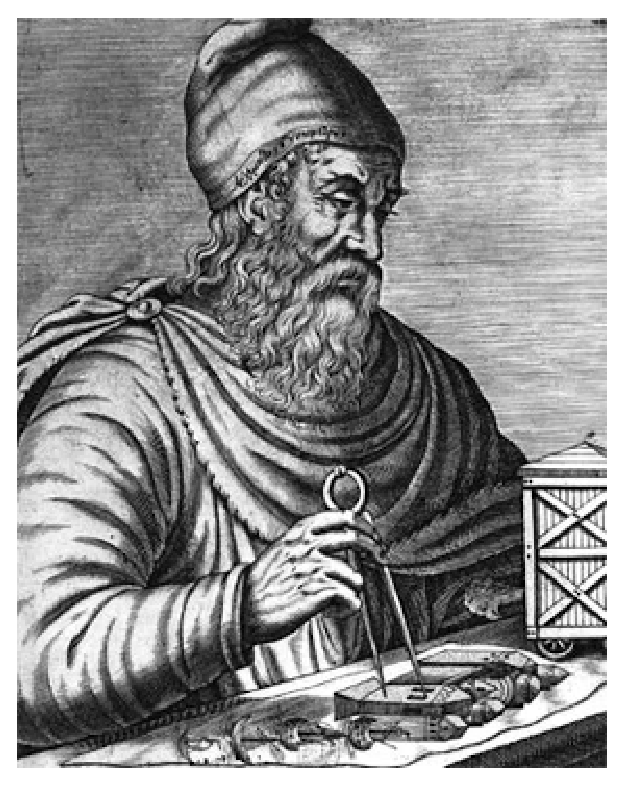
\includegraphics[width=3cm]{Archimede}
      \end{minipage}
      
   \partie[la méthode d'Archimède] \smallskip
      \begin{minipage}{5cm}
         \begin{pspicture}(-2.5,-2.25)(2.5,2.25)
            \pscircle(0,0){2}
            \psline[linewidth=1mm](-2,0)(2,0)
            \psarc[linewidth=1mm,linecolor=red](0,0){2}{0}{180}
            \psarc[linewidth=1mm,linecolor=blue](0,0){2}{180}{0}
            \multido{\r=0+22.5}{16}{\psline(0,0)(2;\r)}
         \end{pspicture}
      \end{minipage}
      \qquad
      \begin{minipage}{10cm}
         \begin{itemize}
            \item Tracer sur une feuille au format A4 un disque de rayon \ucm{6}.
            \item Tracer un diamètre de ce cercle puis repasser en rouge l'un des demi-cercles et en bleu l'autre demi-cercle.
            \item Découper ce cercle en deux parts égales, puis quatre, puis huit, puis seize. Proposer une méthode pour cela (il est possible d'utiliser tout le matériel de géométrie). 
         \end{itemize}
         \begin{enumerate}
            \item Calculer la valeur du périmètre de ce disque : \pf
         \end{enumerate}
      \end{minipage} \\
      \begin{itemize}
         \item Assembler les portions de disque comme sur la {\it figure 1} ci-dessous.
         \item Découper l'un des deux portions de disque des extrémités en deux parts égales.
         \item Coller sur le cahier toutes les portions de disque selon la {\it figure 2}.
         \begin{center}
            \begin{pspicture}(-0.5,-0.5)(14.5,2.5)
               \def\portion{
                  \psline(2;101.25)(0,0)(2;78.75)(0.79,0)
                  \psarc[linewidth=1mm,linecolor=red](0,0){2}{78.35}{101.65}
                  \psarc[linewidth=1mm,linecolor=blue](2;78.75){2}{-101.65}{-78.35}}
               \multido{\n=0+0.79}{8}{\rput(\n,0){\portion}}
               \rput(3,-0.5){\it figure 1}
               \rput(7,1){$\Rightarrow$}
               \multido{\n=8+0.79}{9}{\rput(\n,0){\portion}}
               \psframe*[fillstyle=solid,fillcolor=white,linecolor=white](8,-0.1)(7.5,2.1)
               \psline(8,-0.05)(8,2.05)
               \psframe*[fillstyle=solid,fillcolor=white,linecolor=white](14.32,-0.1)(15.15,2.1)
               \psline(14.32,-0.05)(14.32,2.05)
               \rput(11.5,-0.5){\it figure 2}
            \end{pspicture}
         \end{center}
      \end{itemize}
      \begin{enumerate}
      \setcounter{enumi}{1}
         \item À quoi \og ressemble \fg{} la figure 2 obtenue ? \pf \medskip
         \item En s'appuyant sur les mesures prises sur la figure collée, donner une approximation de son aire : \pf
      \end{enumerate}
         
   \partie[vers la formule de l'aire du disque] \smallskip   
      On considère ici un cercle de rayon $R$ découpé de la même manière que dans la partie B. \\ [2mm]
      \begin{minipage}{9cm} 
         \begin{enumerate}
         \setcounter{enumi}{3}
            \item Sur la figure ci-contre, exprimer la longueur $L$ et la largeur $\ell$ en fonction de $R$ en considérant que la longueur $L$ est presque équivalente à la longueur de la courbe en bleu.
            \item En déduire la formule proposée par Archimède pour l'aire d'un disque : \pf \medskip
            \item Comment cette approximation peut-elle se justifier ?
         \end{enumerate}
      \end{minipage}
      \qquad
      \begin{minipage}{7cm}
         {\psset{unit=0.9}
         \begin{pspicture}(7,-0.5)(14.5,2.5)
            \def\portion{
               \psline(2;101.25)(0,0)(2;78.75)(0.79,0)
               \psarc[linewidth=1mm,linecolor=red](0,0){2}{78.35}{101.65}
               \psarc[linewidth=1mm,linecolor=blue](2;78.75){2}{-101.65}{-78.35}}
            \multido{\n=8+0.79}{9}{\rput(\n,0){\portion}}
            \psframe*[fillstyle=solid,fillcolor=white,linecolor=white](8,-0.1)(7.5,2.1)
            \psline(8,-0.05)(8,2.05)
            \psframe*[fillstyle=solid,fillcolor=white,linecolor=white](14.32,-0.1)(15.15,2.1)
            \psline(14.32,-0.05)(14.32,2.05)
            \rput(11.5,-0.5){$L=\dots$}
            \rput{90}(7.5,0.75){$\ell =\dots$}
         \end{pspicture}}
      \end{minipage}

      
